%%
%% This is file `example/ch_intro.tex',
%% generated with the docstrip utility.
%%
%% The original source files were:
%%
%% install/buptgraduatethesis.dtx  (with options: `ch-intro')
%%
%% This file is a part of the example of BUPTGraduateThesis.
%%

\chapter{探索使用数据集全局信息指导神经网络Dropout方式}

\section{引言}

\section{GI-Dropout方法}
我们方法背后的直觉非常简单。
由于神经网络旨在捕获语义特征并根据其语义特征对句子进行分类,我们鼓励模型尽可能的学习更多的特征(尤其是那些不那么显著的特征)。我们的方法是,通过计算每个单词对分类的显著性,在神经网络训练的过程中,将显著性高的单词以一定的概率丢弃,从而迫使模型多去学习那些不显著的特征。
有一些特征非常的具有区分性,使得模型可以很容易地学习它们。但是,一个句子可能具有不止一个有助于类别预测的特征。
例如,在``The story is sad and very boring''中,``boring''具有强烈的极性并表示负面情绪。
而由于``boring''的强烈影响,神经网络会``偷懒'',因为他只要看见``boring''就能做正确的判断,这使得神经网络将没有动力去学习同样有助于分类的``sad''特征。
基于这个想法,我们提出了GI-Dropout中,在训练过程中,使得显著性较高的单词有一定的概率被丢弃,从而迫使模型学习其他特征,而在预测时,使用全部特征,从而获得更好的性能。
\begin{figure}[!t]
\centering
  \includegraphics[width=\linewidth]{figure/gi.pdf}
  \caption{GI-Dropout方法. 在这个例子中,单词``boring''的词向量被丢弃因而被设为了0向量,而单词``sad''的向量保留了}
  \label{fig:model}
\end{figure}



\section{实验}
\subsection{数据集}
\begin{table}[!t]
% \renewcommand{\arraystretch}{1.3}
\centering
\begin{tabular}{c c c c c c}
\hline
\bfseries 数据集 & 类别数 & 句子长度 & 数据集大小 & 词表大小  & 测试集\\
\hline
MR & 2 & 20 & 10662 & 18765 &  交叉验证\\
SST-1 & 5 & 18 & 11855 & 17836  & 2210\\
SST-2 & 2 & 19 & 9613 & 16185  & 1821\\
Subj & 2 & 23 & 10000 & 21323  & 交叉验证\\
TREC & 6 & 10 & 5952 & 9592  & 500\\
CR & 2 & 19 & 3775 & 5340  & 交叉验证\\
MPQA & 2 & 3 & 10606 & 6246 & 交叉验证\\
\hline
\end{tabular}
\caption{\ 数据集介绍整体情况概述,交叉验证指该数据集没有明确区分训练集、测试集,因此我们用交叉验证的方式进行结果检验。}
\label{table: dataset summary}
\end{table}


\subsection{实验设置}

\subsection{实验结果}

\begin{table*}[t]
\begin{small}
% \begin{singlespace}
\tabcolsep=0.11cm

% \renewcommand{\arraystretch}{1.3}
\centering
\begin{tabular}{c |ccccccc}
\hline
\bfseries Model             & MR   & SST-1 & SST-2 & Subj & TREC &  CR  & MPQA\\
\hline
CNN-non-static & 81.5 & 48.0  & 87.2  & 93.4 & 93.6 & 84.3 & 89.5\\
\hline
CNN-reproduce       & 81.4 & 47.8  & 87.5  & 93.0 & 92.4 & 84.3 & 89.6\\
CNN-Dropout-same (p)       &  81.5(0.1) & 48.5(0.1)  & 87.6(0.1)  & 93.5(0.2) & 92.9(0.1)& 84.5(0.5) & 87.4(0.1)\\

CNN-GI-Dropout ($\beta$) & \textbf{81.9}(0.87) & \textbf{49.0}(0.95)  & \textbf{88.1}(0.98)  & \textbf{93.4}(0.91) & \textbf{93.2}(0.83) & \textbf{85.1}(0.87) & \textbf{89.8}(0.98)\\

\hline
\hline
RNN-baseline & 82.1 & 49.7  & 89.7  & 93.6 & 92.6 & 84.1 & 89.6\\
RNN-Dropout-same (p) & 82.2(0.2) & 51.9(0.1)  & 90.1(0.1)  & 93.9(0.1) & 93.4(0.2) & 84.2(0.1) & \textbf{89.7}(0.1)\\
RNN-GI-Dropout ($\beta$) & \textbf{82.5}(0.87) & \textbf{54.1}(0.95)  & \textbf{90.4}(0.95)  & \textbf{94.2}(0.98) & \textbf{94.8}(0.95) & \textbf{84.7}(0.91) & \textbf{89.7}(0.98)\\

\hline
\hline
MVCNN & - & 49.6 & \underline{89.4} & 93.9 & - & - & -\\ 
MGNC-CNN & - & 48.7 & 88.3 & \underline{94.1} & 95.5 & - & -\\ 
CNN-Rule & 81.7 & - & 89.3 & - & - & 85.3 & -\\ 
Semantic-CNN & 82.1 & 50.8 & 89.0 & 93.7 & 94.4 & \underline{86.0} & \underline{89.3}\\ 
combine-skip & 76.5 & - & - & 93.6 & 92.2 & 80.1 & 87.1\\ 
DSCNN & \underline{82.2} & 50.6 & 88.7 & 93.9 & \underline{95.6} & - & -\\ 
Paragraph Vector & 74.8 & 48.7 & 87.8 & 90.5 & 91.8 & 78.1 & 74.2\\ 
NBSVM & 79.4 & - & - & 93.2 & - & 81.8 & 86.3\\ 
Tree LSTM & - & \underline{51.0} & 88.0 & - & - & - & -\\ 
\hline
\end{tabular}

\caption{Effectiveness of GI-Dropout.
Dropout-same means dropping units with the same probability.
Results also include: MVCNN \cite{yin2015multichannel}, MGNC-CNN \cite{zhang2016mgnc}, CNN-Rule \cite{hu2016harnessing}, Semantic-CNN \cite{li2017initializing}, combine-skip \cite{kiros2015skip}, combine-skip \cite{kiros2015skip}, DSCNN \cite{zhang2016dependency}, Paragraph Vector \cite{le2014distributed}, NBSVM \cite{wang2012baselines} and Tree LSTM \cite{tai2015improved}.
}

\label{table: result}
\qquad
% \end{singlespace}

\end{small}
\end{table*}


\subsection{GI-Dropout的效果}

\section{结果深入分析}

\subsection{GI-dropout 帮助模型学习不显著特征}
\begin{table}[!t]
% \renewcommand{\arraystretch}{1.3}
\centering
\begin{tabular}{c | c c}
\hline
\bfseries Top-k &  CNN baseline &  GI-Dropout in CNN\\
\hline
0 & 87.5 & 88.1  \\
50 & 87.1 & 87.9  \\
100 & 86.7 & 87.9  \\
200 & 86.1 & 87.5  \\
500 & 84.7 & 86.6  \\
1000 & 81.7 & 84.0 \\

\hline
\hline
\end{tabular}
\caption{在SST-2数据集中,当我们移去top-k关键词后的准确率下降趋势。}
\label{table: decline-SST-2}
\end{table}
为了测试该方法是否确实有助于模型学习不明显的特征,我们进行了如下实验,即从“ SST-2”的测试用例中删除了前k个显著词(具有最高重要分数的词),观察他的效果。
结果显示在表\ref{table: decline-SST-2}中。
我们可以观察到CNN baseline模型对显著特征更为敏感,而相反,即使删除了前1000个显著词,引入了GI-Dropout的模型仍然可以取得相对较好的结果。
因此,GI-Dropout可以帮助模型更加关注那些不显著的特征。


\subsection{GI-dropout 帮助模型减少对显著特征的过拟合}
我们都知道,频繁出现的一些单词很容易使模型专注于某一些特征,并且在全连接层只激活分数较高的部分单元。我们从测试用例中挑选了部分baseline模型做错,而GI-Dropout模型做对的用例,并进行进一步分析。示例中,\textbf{加粗}的单词代表那些有着高分的显著词, 例如在\textbf{positive}中出现了159次而只在\textbf{negative}出现了5次的``pretentious". \underline{下划线}的单词代表了那些非显著的,但是也对分类有贡献的单词。 

\textbf{(1)}  \textit{provide -lrb- s -rrb- nail-biting suspense and credible characters \underline{without} relying on technology-of-the-moment technique or \textbf{pretentious} dialogue.}

\textbf{(2)}  \textit{the screenplay \underline{sabotages} the movie's \textbf{strengths} at almost every juncture.} 

\textbf{(3)}  \textit{this is \underline{cool}, \underline{slick} stuff, ready to \underline{quench} the thirst of an audience that \textbf{misses} the summer blockbusters.} 

baseline模型倾向于关注那些非常显著且起决定作用的特征。如例1的\textbf{``pretentious"} (消极性), 例2的\textbf{``strengths"} (积极性)和例3的\textbf{``miss"} (消极性)。由于对这些非常显著特征的过拟合,且忽视了例1的\textbf{``without"}, 例2的\textbf{``sabotages"}, \textbf{``cool"}, \textbf{``slick"} 和例3的 \textbf{``quench"},baseline模型没有好好利用整句话中的所有信息,导致分类错误。
当引入了GI-dropout方法后,模型不但能学会到\textbf{``strengths"}这种显著特征,也会学习到\textbf{``sabotages"}这种不显著特征,使得该模型能够就行正确的分类。

\textbf{$\beta$ 和正确率的关系}

\begin{figure}[!t]
\centering
  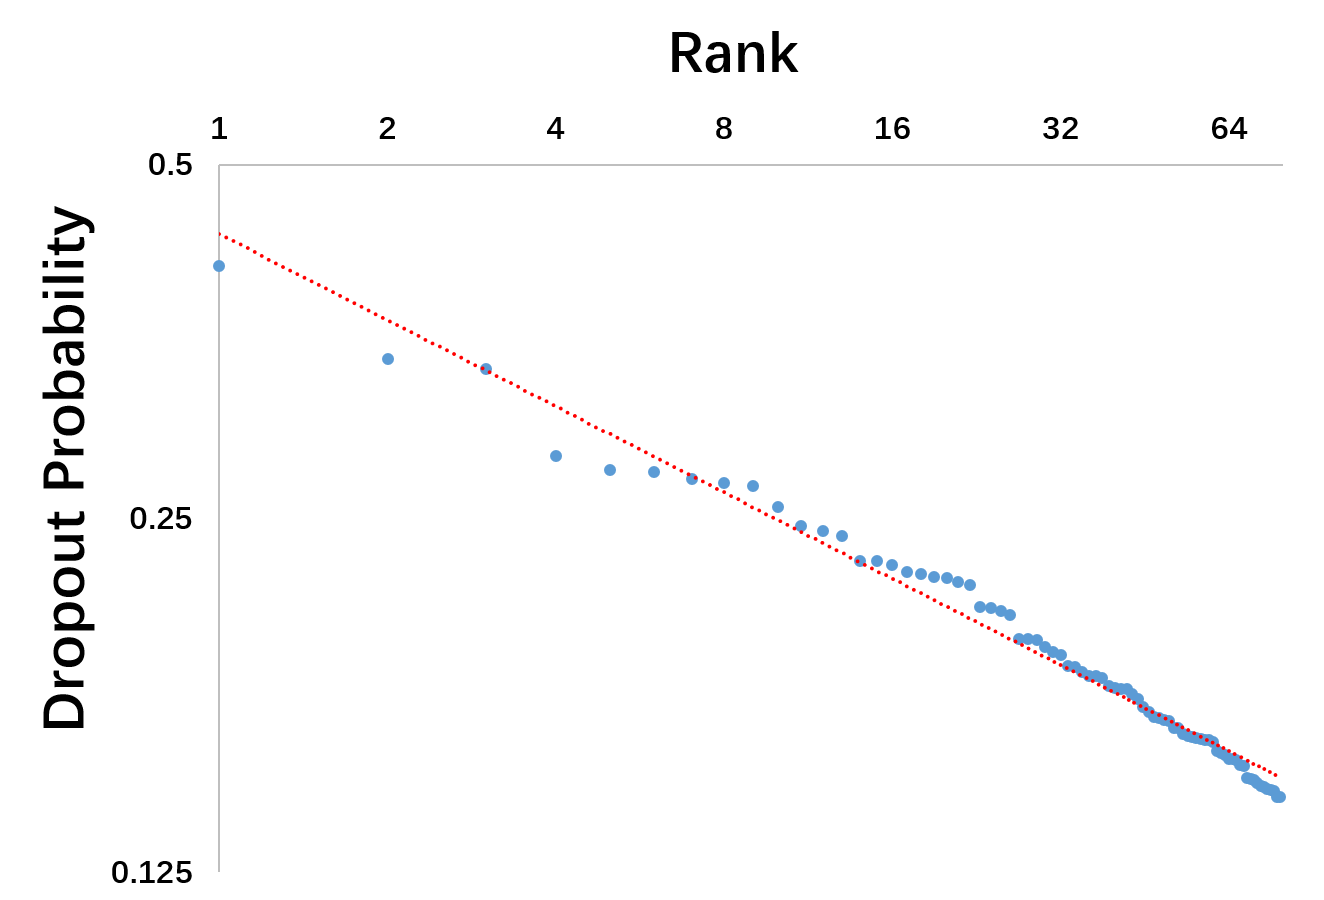
\includegraphics[width=\linewidth]{figure/zipf.png}
  \caption{当$\beta = 0.95$时,数据集SST-1中,GI-Dropout中单词概率和频率排名的关系。}
  \label{fig:zipf}
\end{figure}

\begin{table}[!t]
% \renewcommand{\arraystretch}{1.3}
\centering
\begin{tabular}{c | c c}
\hline
\bfseries $\beta$ & CNN &  RNN\\
\hline
0.98 ($10^{-0.01}$) & 48.8 & 51.9 \\
0.95 ($10^{-0.02}$) & \textbf{49.0} & \textbf{54.1} \\
0.91 ($10^{-0.04}$) & 48.0 & 51.8 \\
0.87 ($10^{-0.06}$) & 48.1 & 52.4 \\
0.83 ($10^{-0.08}$) & 47.4 & 51.4 \\

\hline
\hline
\end{tabular}
\caption{$\beta$ and accuracy in SST-1. }
\label{table: SST-1}
\end{table}

此外,我们对于超参$\beta$的取值进行了分析。如图\ref{fig:zipf}所示,当$\beta$的值为0.95时,在数据集SST-1中,每个单词的dropout概率和他的排名近似符合Zipf's Law。事实上,在每一个数据集中,都存在一个准确的$\beta$,使得单词的dropout的概率和其在数据集中词频的排名近似符合Zipf's Law,且这个$\beta$就是让模型达到最好效果的$\beta$。我们认为,这是因为Zipf's Law反映了词重要性和词频的客观规律,根据这一定律设置$\beta$值,会更好的体现数据集的特性。为此,我们做了进一步实验,表\ref{table:SST-1}证明了我们的猜想,无论是CNN还是RNN,都是$\beta$值为0.95的时候,GI-Dropout方法取得了最好的效果。


\begin{enumerate}
\item 第二章介绍……
\item ……
\end{enumerate}

\chapterbib

